\documentclass[tikz]{standalone}
%\usetikzlibrary{calc}
\begin{document}


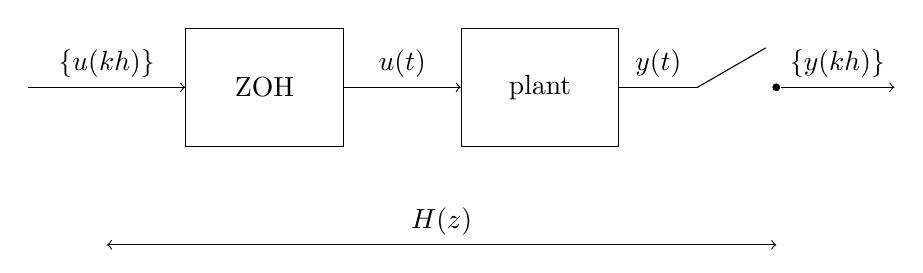
\begin{tikzpicture}[node distance=3cm]
  \node[coordinate] (input) {};
  \node[coordinate, right of=input, node distance=1cm] (Hleft) {};
  \node[rectangle, draw, minimum height=15mm, minimum width=20mm, right of=input] (zoh) {ZOH};
  \node[rectangle, draw, minimum height=15mm, minimum width=20mm,right of=zoh, node distance=35mm] (plant) {plant};
  \node[coordinate, right of=plant, node distance=20mm] (sample) {};
  \node[circle, fill, inner sep=1pt, right of=sample, node distance=10mm] (contact) {};
  \node[coordinate, right of=contact, node distance=15mm] (output) {};

  \draw[->] (input) -- node[above] {$\{u(kh)\}$} (zoh);
  \draw[->] (zoh) -- node[above] {$u(t)$} (plant);
  \draw[-] (plant) -- node[above] {$y(t)$} (sample);
  \begin{scope} [rotate=30] \draw (sample) -- ++(10mm, 0); \end{scope}
  \draw[->] (contact) -- node[above] {$\{y(kh)\}$} (output);

  \node[coordinate, below of=Hleft, node distance=2cm] (Hstart) {};
  \node[coordinate, below of=contact, node distance=2cm] (Hend) {};

  \draw[<->] (Hstart) -- node [above] {$H(z)$} (Hend);
\end{tikzpicture}
\end{document}
